% arara: pdflatex
\documentclass{beamer}
\usepackage[utf8]{inputenc}
\usepackage{hyperref}

\title{\Huge\texttt{vim} \\ \normalsize ``Who needs a mouse?''}
\author{Nicolas Dorrmann}
\date{04. Nov. 2020}

\begin{document}

\frame{\titlepage}

\begin{frame}
    \frametitle{History and Design Philosophy}
    \begin{itemize}
        \item Developed by Bram Moolenaar, initially released in 1991.
        \item Successor to \texttt{vi} (\textbf{v}isual \textbf{i}nterface for line editor \texttt{ex}).
        \item Editing works entirely over keyboard, most commands are easily reachable over home row.
        \item Plugins (written in \texttt{VimScript}) \textit{can} provide functionality similar to an IDE.
    \end{itemize}
\end{frame}
\begin{frame}
    \frametitle{But why?}
    \begin{itemize}
        \item It's everywhere (if you want it) --- a lot of software has the option of using \texttt{vim} keybindings.
        \begin{description}
            \item [\texttt{qutebrowser}]  webbrowser
            \item [\texttt{vifm}]         filemanager
            \item [\texttt{IdeaVim}]      \texttt{vim} keybindings for JetBrains IDEs
            \item [\texttt{ExcelLikeVim}] \texttt{vim} keybindings for MS Excel (yes, seriously)
        \end{description}
        \item It's versatile --- lightweight text editor or almost-universal IDE (or anything in between).
        \item It's ``intuitive'' --- after getting used to it, you can use \texttt{vim} almost like a language.
    \end{itemize}
\end{frame}
\begin{frame}
    \frametitle{Basics - The Interface}
    \begin{center}
    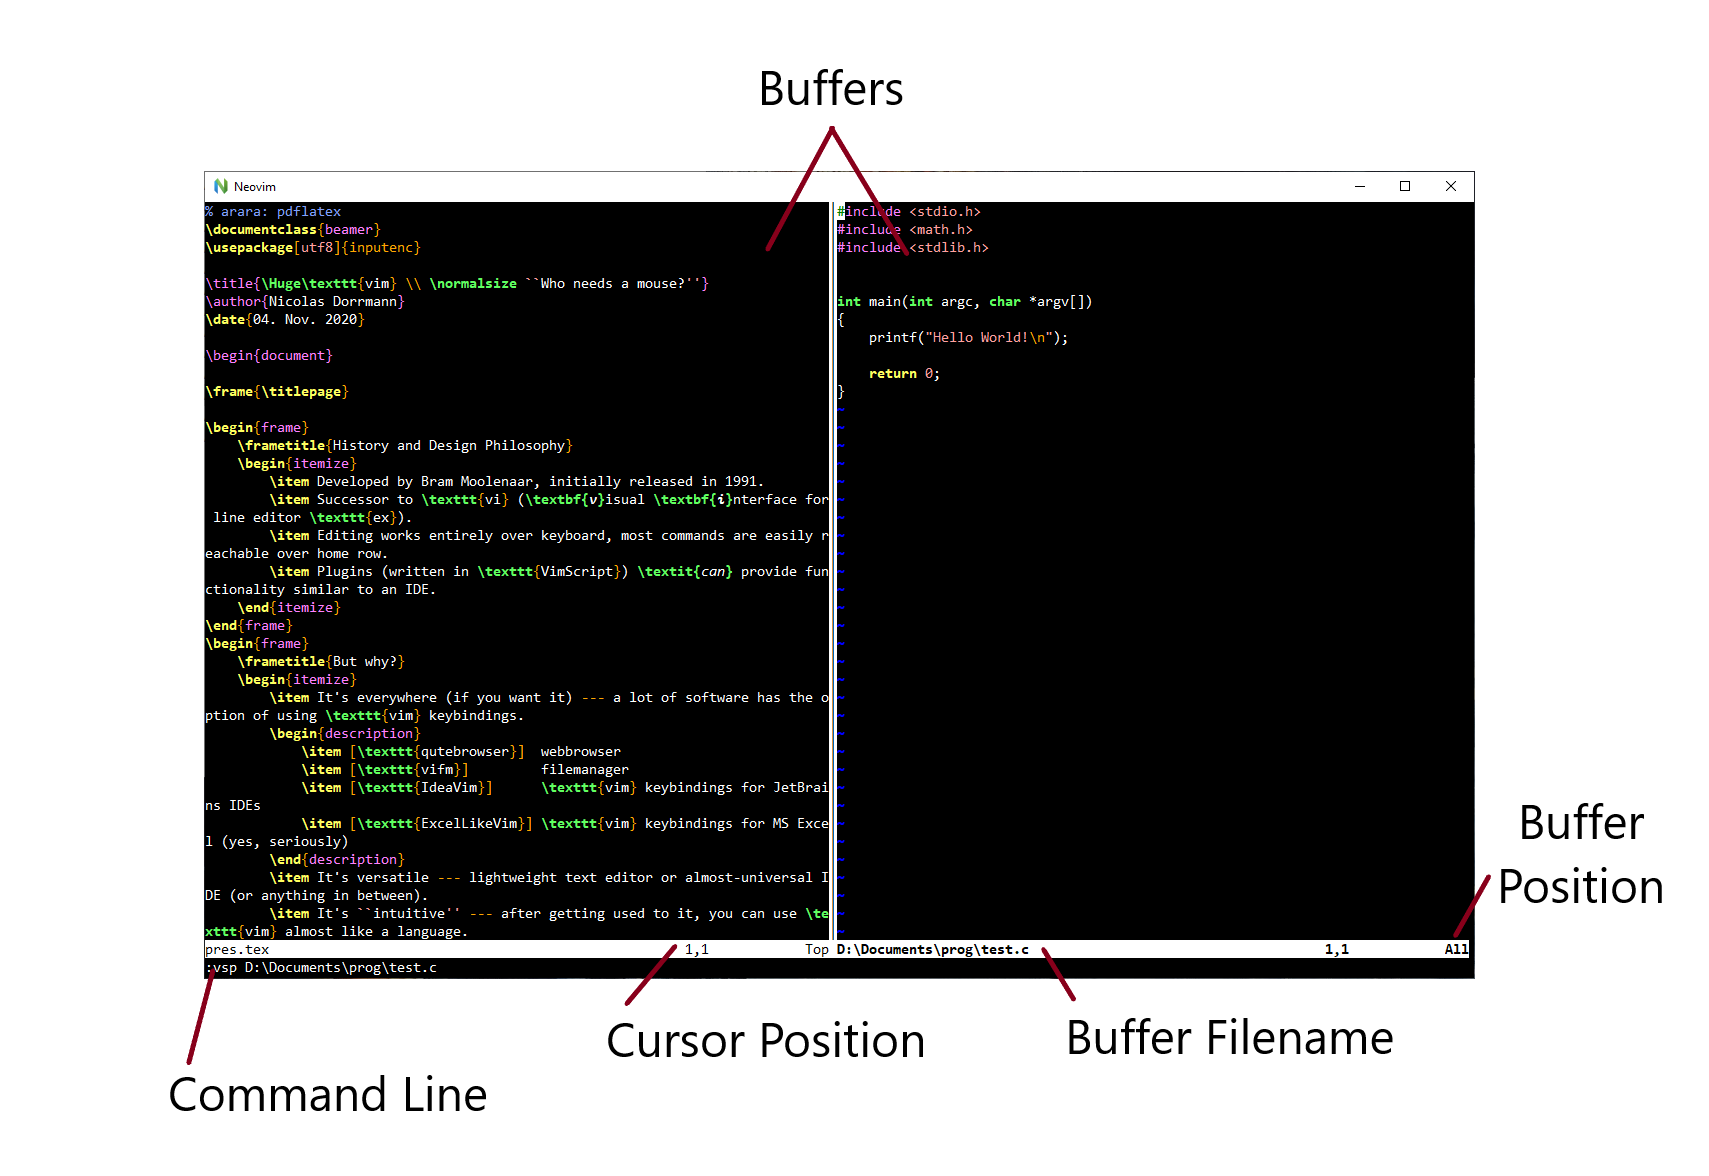
\includegraphics[width=\textwidth]{graphics/vim_screen_annotated.png}
    \end{center}
\end{frame}
\begin{frame}
    \frametitle{Basics - Modes}
    \begin{description}
        \item [\texttt{NORMAL}]  navigate within the file, issue text commands (yank/change/delete)
        \item [\texttt{COMMAND}] open, close, or save a file
        \item [\texttt{INSERT}]  direct input (i.\ e.\ actually typing text)
        \item [\texttt{VISUAL}]  text highlighting, text blocking
    \end{description}
    \vspace{0.5cm}
    \begin{center}
        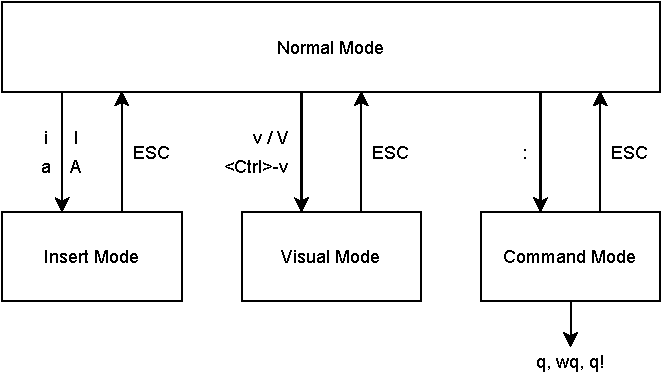
\includegraphics[width=0.6\textwidth]{graphics/vim_modes.pdf}
    \end{center}
\end{frame}
\begin{frame}
    \frametitle{Basics}
    \begin{itemize}
        \item Actions (``verbs'')
        \begin{description}
            \item [\textbf{y}ank]   copy a movement
            \item [\textbf{c}hange] replace object with a new object
            \item [\textbf{d}elete] remove an object
        \end{description}
        \item Modifiers
        \begin{description}
            \item [\texttt{NUM}] number of objects to perform action on
            \item [\texttt{i}]   perform action \textbf{i}nside an object
            \item [\texttt{a}]   perform action \textbf{a}round an object
            \item [\texttt{t}]   perform action up \textbf{t}o an object
            \item [\texttt{f}]   perform action up to and including an object
        \end{description}
        \item Text Objects (``nouns'')
        \begin{description}
            \item [\textbf{w}ord]      string of non-whitespace characters surrounded by whitespace
            \item [\textbf{s}entence]  ends with \texttt{!}, \texttt{?}, \texttt{.} followed by newline
            \item [\textbf{p}aragraph] consists of several sentences, delimited by empty lines
        \end{description}
    \end{itemize}
\end{frame}
\begin{frame}
    \frametitle{Commands}
    \begin{itemize}
        \item Basic commands have the form \texttt{Action} --- \texttt{Modifier} --- \texttt{Object}
        \item Examples
        \begin{description}
            \item [\texttt{y2w}] copy the next two words
            \item [\texttt{dis}] delete the current sentence (i.\ e.\ the sentence the cursor is in)
            \item [\texttt{cp}]  change (i.\ e.\ delete and enter \texttt{INSERT} mode) the current paragraph
        \end{description}
    \end{itemize}
\end{frame}
\begin{frame}
    \frametitle{Search and Replace}
    \begin{itemize}
        \item Search
        \begin{itemize}
            \item Forward search with \texttt{/string}. Backward search with \texttt{?string}.
            \item Next result with \texttt{n}, previous with \texttt{N}.
        \end{itemize}
        \item Search and Replace (\texttt{substitute})
        \begin{itemize}
            \item Basic syntax: \texttt{:[range]s/search/replace/}
            \item \texttt{[range]} is a line, range of lines (\texttt{start, end}), or entire buffer (\texttt{\%}).
            \item Global replace with \texttt{g} or with confirmation (\texttt{gc}).
        \end{itemize}
    \end{itemize}
\end{frame}
\begin{frame}
    \frametitle{Regular Expressions}
    \begin{description}
        \item [\texttt{.}] match one of any character
        \item [\texttt{[range]}] matches any one of the characters in \texttt{range}
        \item [\texttt{*}] match arbitrary many repetitions of preceding character
        \item [\texttt{\textbackslash+}] match one or more of the preceding character
        \item [\texttt{\textbackslash=}] match none or one of the preceding character
        \item [\texttt{\{m,n\}}] between \texttt{m} and \texttt{n} repetitions
        \item [\texttt{\textasciicircum}] match start of a line
        \item [\texttt{\$}] match end of a line
    \end{description}
\end{frame}
\begin{frame}
    \frametitle{\texttt{.vimrc} / \texttt{init.vim}}
    \begin{itemize}
        \item Configuration file for \texttt{vim} settings.
        \item Written in \texttt{VimScript}, an interpreted programming language.
        \item Read and executed at editor startup (provided it exists).
        \item Allows various customization options:
        \begin{itemize}
            \item font, syntax highlighting and color scheme
            \item define or redefine keybindings
            \item modify various preset options
        \end{itemize}
    \end{itemize}
\end{frame}
\begin{frame}
    \frametitle{VimScript Basics}
    \begin{description}
        \item [\texttt{(i/c/v/n)map}] (re)map a key combination
        \item [\texttt{set}] (re)define an option
        \item [\texttt{let}] (re)define a variable
        \item [\texttt{source}] ``include'' an additional \texttt{.vim} file
        \item [\texttt{:help xyz}] open documentation on \texttt{xyz}
    \end{description}
\end{frame}
\begin{frame}
    \frametitle{Plugins and Plugin Managers}
    \begin{itemize}
        \item \href{http://vimawesome.com/} --- An excellent resource for \texttt{vim} plugins.
        \item Plugin Manager
        \begin{itemize}
            \item \texttt{pathogen.vim} -- minimalist, simple to use, requires manual installation/deinstallation
            \item \texttt{vundle} -- requires listing all plugins in \texttt{.vimrc}
            \item \texttt{vim-plug} -- similar to \texttt{vundle}
        \end{itemize}
    \end{itemize}
\end{frame}
\begin{frame}
    \frametitle{Tutorial: Setting up a Productive \texttt{Neovim} Environment}
    In this tutorial, we will do the following:
    \begin{enumerate}
        \item Configure the \texttt{pathogen.vim} plugin manager.
        \item Install the \texttt{Dracula} color scheme and \texttt{UltiSnips} snippet manager.
        \item Create a few snippets for quickly creating Java classes.
    \end{enumerate}
\end{frame}
\end{document}

